\documentclass[border=10pt]{standalone}
\usepackage{xcolor}
\usepackage{tikz}
\usepackage{pgfplots}
\pgfplotsset{compat=1.18}

\definecolor{INK}{HTML}{1A1A2E}
\definecolor{BG}{HTML}{FAFAFA}
\definecolor{SUB}{HTML}{555566}
\definecolor{BURST}{HTML}{D81159}
\definecolor{SEQ}{HTML}{2A9D8F}

\begin{document}
\pagecolor{BG}
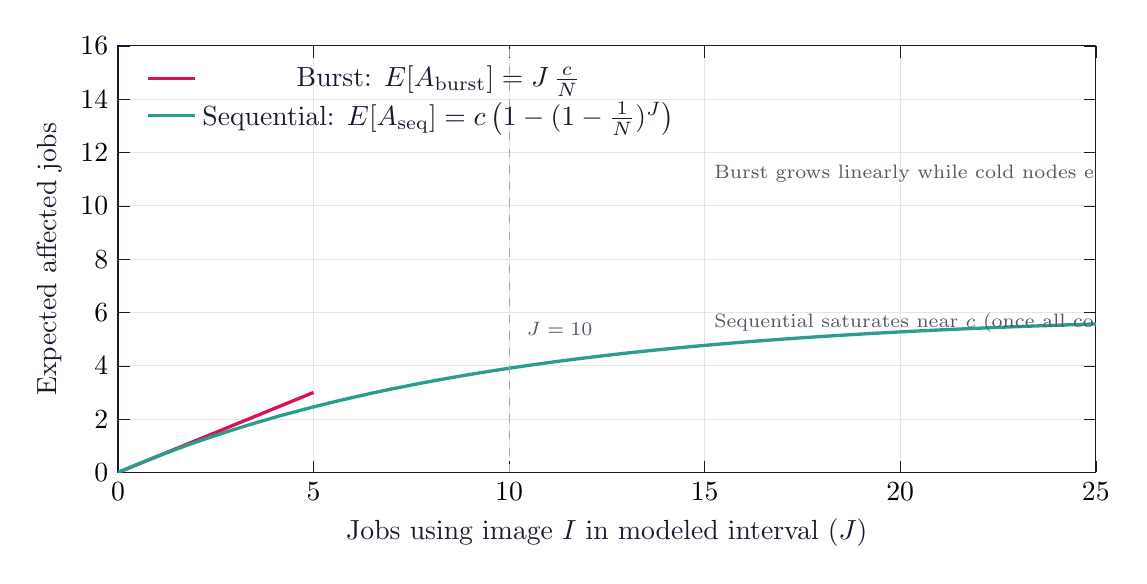
\begin{tikzpicture}
\begin{axis}[
  width=14cm,
  height=7cm,
  xlabel={Jobs using image $I$ in modeled interval ($J$)},
  ylabel={Expected affected jobs},
  xmin=0, xmax=25,
  ymin=0, ymax=16,
  xtick={0,5,10,15,20,25},
  ytick={0,2,4,6,8,10,12,14,16},
  grid=major,
  grid style={draw=gray!20},
  axis line style={draw=INK},
  tick style={draw=INK},
  xlabel style={text=INK},
  ylabel style={text=INK},
  legend style={draw=none, fill=none, text=INK, at={(0.02,0.98)}, anchor=north west},
]
  % Example parameters from paper-style toy setup: N=10, c=6
  \addplot[very thick, BURST] {0.6*x};
  \addlegendentry{Burst: $E[A_{\mathrm{burst}}]=J\,\frac{c}{N}$}

  \addplot[very thick, SEQ, domain=0:25, samples=200] {6*(1 - (1-1/10)^x)};
  \addlegendentry{Sequential: $E[A_{\mathrm{seq}}]=c\left(1-(1-\frac1N)^J\right)$}

  \addplot[dashed, gray!70] coordinates {(10,0) (10,16)};
  \node[font=\scriptsize, text=SUB, anchor=west] at (axis cs:10.2,5.4) {$J=10$};

  \node[font=\scriptsize, text=SUB, anchor=west] at (axis cs:15,11.2)
    {Burst grows linearly while cold nodes exist};
  \node[font=\scriptsize, text=SUB, anchor=west] at (axis cs:15,5.6)
    {Sequential saturates near $c$ (once all cold nodes are hit)};
\end{axis}
\end{tikzpicture}
\end{document}
